\subsection{Passage à l'échelle}
Comme dit dans le chapitre précédent, l'algorithme du GMRES se parallélise bien parce qu'il est essentiellement composé d'opérations sur des vecteurs.
%
L'opération la plus coûteuse est le produit d'une matrice par un vecteur (SpMV).
%
Notre implémentation du SpMV est optimisée pour prendre en compte la structure bloc des entrées de la matrice quand le nombre de variables primaires est supérieur à 1.
%
Dans ce cas, nous pouvons réutiliser des données en cache.
%
Malgré ces optimisations, le SpMV est toujours limité par la bande passante mémoire.
%
Les courbes d'accélération du SpMV nous montrent que le gain de performance n'est pas linéaire avec le nombre de coeurs (Fig.~\ref{fig:res_spmv_omp_rostand})..
%
Le constat est même pire que ça, on arrive difficilement à une accélération de 2 sur 12 coeurs lorsqu'on utilise une seule variable primaire.
%
Si l'on regarde les compteurs matériels, on s'aperçoit que la moitié de la bande passante de chaque banc NUMA est utilisée par des accès distant.
%
Donc environ la moitié des accès mémoires sont faits une plus grande latence.

%   (-_-)   %
\begin{figure}
  \centering
  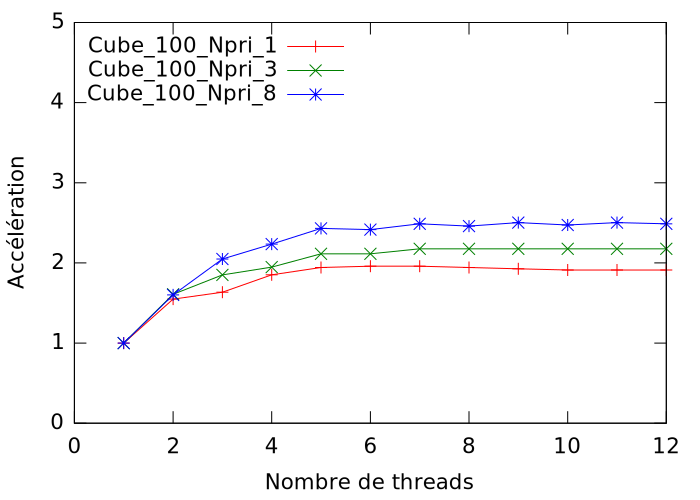
\includegraphics[width=0.7\textwidth]{res_spmv_omp}
  \caption{Accélération du produit matrice vecteur creux sur Rostand en mémoire partagée.}
  \label{fig:res_spmv_omp_rostand}
\end{figure}
